% Flipped classroom module for the AI for Educators seminar (workshop use).
% Included from seminar_ai_for_educators_content.tex by one \input line: comment that line
% with % to switch the whole module off. Four sections: Flipped, LMS, Build, Activity.
% CheatSheet-safe: no floats, the one wide table is wrapped in \resizebox.

\section[Flipped]{The Flipped Classroom}

%%%%%%%%%%%%%%%%%%%%%%%%%%%%%%%%%%%%%%%%%%%%%%%%%%%%%%%%%%%%%%%%%%%%%%%%%%%%%%%%%%
\begin{frame}[fragile]\frametitle{}
\begin{center}
{\Large The Flipped Classroom}

\medskip
{\small (Content first at home, discussion and depth in class)}
\end{center}
\end{frame}

%%%%%%%%%%%%%%%%%%%%%%%%%%%%%%%%%%%%%%%%%%%%%%%%%%%
\begin{frame}[fragile]\frametitle{What Is a Flipped Classroom?}
\begin{itemize}
\item \textbf{Traditional:} the teacher explains new content in class; students practise alone at home.
\item \textbf{Flipped:} students meet the content first, on their own time; class time goes to discussion, problems and advanced ideas.
\item The lecture moves out of the classroom. The teacher stays in the room for the hard part: questions, misconceptions, application.
\item The idea is old. What changed is how cheaply a teacher can now prepare the pre-class material.
\end{itemize}
\end{frame}

%%%%%%%%%%%%%%%%%%%%%%%%%%%%%%%%%%%%%%%%%%%%%%%%%%%
\begin{frame}[fragile]\frametitle{Why AI Makes Flipping Practical}
\begin{itemize}
\item The classic objection: preparing good reading, notes, diagrams and quizzes for every topic takes too much teacher time.
\item AI is good at exactly this first-draft work: structure a syllabus, draft notes, suggest diagrams, write exercises and quiz items.
\item The teacher keeps the judgement: what to include, what is correct, what suits these students.
\item Result: the teacher spends hours reviewing material, not days writing it.
\end{itemize}
\end{frame}

%%%%%%%%%%%%%%%%%%%%%%%%%%%%%%%%%%%%%%%%%%%%%%%%%%%
\begin{frame}[fragile]\frametitle{What Class Time Becomes}
\begin{itemize}
\item \textbf{Start with a check:} a short quiz or question on the pre-class material shows who read it and what confused them.
\item \textbf{Discuss the confusing parts:} the teacher spends time where students actually struggled.
\item \textbf{Apply:} problems, case studies, group work, debate, hands-on tasks.
\item \textbf{Go further:} advanced extensions that a plain lecture never had time for.
\end{itemize}
\end{frame}

%%%%%%%%%%%%%%%%%%%%%%%%%%%%%%%%%%%%%%%%%%%%%%%%%%%
\begin{frame}[fragile]\frametitle{Route 1: A Plain Textbook}
\begin{itemize}
\item Give the students the chapters to read before each class: the simplest route, with no technology to set up.
\item Name the exact chapters and pages, and add three guiding questions to answer while reading.
\item \textbf{Strength:} authoritative, already written, free to the teacher.
\item \textbf{Weakness:} no tracking, no interaction, and a student can skip it without anyone noticing.
\end{itemize}
\end{frame}

%%%%%%%%%%%%%%%%%%%%%%%%%%%%%%%%%%%%%%%%%%%%%%%%%%%
\begin{frame}[fragile]\frametitle{Route 2: Your Own Course Notes}
\begin{itemize}
\item Hand out notes written for \emph{your} syllabus and \emph{your} students, in your own order and level.
\item AI drafts the notes from your syllabus; you correct and localise them. Share as PDF or a printed booklet.
\item \textbf{Strength:} matches your course exactly; examples can use local context and language.
\item \textbf{Weakness:} you must keep them accurate and up to date, and there is still no tracking.
\end{itemize}
\end{frame}

%%%%%%%%%%%%%%%%%%%%%%%%%%%%%%%%%%%%%%%%%%%%%%%%%%%
\begin{frame}[fragile]\frametitle{Route 3: A Curated YouTube Playlist}
\begin{itemize}
\item Collect the best existing videos on each topic into one ordered playlist, with a note on what to watch for.
\item Add a question sheet: three questions per video, answered before class.
\item \textbf{Strength:} excellent explanations already exist, and students can pause and replay.
\item \textbf{Weakness:} videos vary in level and accuracy; links disappear; ads and distractions follow.
\end{itemize}
\end{frame}

%%%%%%%%%%%%%%%%%%%%%%%%%%%%%%%%%%%%%%%%%%%%%%%%%%%
\begin{frame}[fragile]\frametitle{Route 4: A Learning Management System}
\begin{itemize}
\item An LMS holds readings, videos, exercises and quizzes in one place, in a fixed order.
\item It records who opened what, who attempted each quiz and what they scored, so the teacher sees problems before class.
\item Quizzes are graded automatically, with feedback shown straight away.
\item \textbf{Cost:} setup and hosting effort. The next section compares the two main open platforms.
\end{itemize}
\end{frame}

%%%%%%%%%%%%%%%%%%%%%%%%%%%%%%%%%%%%%%%%%%%%%%%%%%%
\begin{frame}[fragile]\frametitle{Choosing a Route}
\begin{center}
\resizebox{\linewidth}{!}{%
\begin{tabular}{lcccc}
\toprule
 & Textbook & Notes & YouTube & LMS \\
\midrule
Teacher effort & Low & Medium & Low & High \\
Matches your syllabus & Partly & Fully & Partly & Fully \\
Interactive & No & No & Little & Yes \\
Tracks students & No & No & No & Yes \\
Setup needed & None & None & None & Server or host \\
\bottomrule
\end{tabular}}
\end{center}
\begin{itemize}
\item These routes combine well: an LMS unit can hold your notes, a video and a quiz together.
\end{itemize}
\end{frame}

\section[LMS]{LMS Platforms}

%%%%%%%%%%%%%%%%%%%%%%%%%%%%%%%%%%%%%%%%%%%%%%%%%%%%%%%%%%%%%%%%%%%%%%%%%%%%%%%%%%
\begin{frame}[fragile]\frametitle{}
\begin{center}
{\Large Open edX and Moodle}

\medskip
{\small (The two main open-source LMS platforms)}
\end{center}
\end{frame}

%%%%%%%%%%%%%%%%%%%%%%%%%%%%%%%%%%%%%%%%%%%%%%%%%%%
\begin{frame}[fragile]\frametitle{Open edX and Moodle: Side by Side}
\begin{center}
\resizebox{\linewidth}{!}{%
\begin{tabular}{lll}
\toprule
 & Open edX & Moodle \\
\midrule
Licence & Open source, no fee & Open source, no fee \\
Built for & Courses at scale, MOOC style & Classes and blended learning \\
Course structure & Section, subsection, unit & Topics, activities, resources \\
Authoring & Studio web editor, OLX import and export & In-page editor, many activity types \\
Quizzes & Built-in problem types, instant feedback & Rich question bank, many types \\
Extensions & XBlocks, plugins & Very large plugin library \\
Setup effort & Higher, container-based & Lower, runs on a standard web host \\
Typical users & Universities, programmes, companies & Schools, colleges, universities \\
\bottomrule
\end{tabular}}
\end{center}
{\footnotesize Features and requirements change between releases: re-check each project's current documentation before choosing.}
\end{frame}

%%%%%%%%%%%%%%%%%%%%%%%%%%%%%%%%%%%%%%%%%%%%%%%%%%%
\begin{frame}[fragile]\frametitle{Open edX: Free Software, Not Free Hosting}
\begin{itemize}
\item The Open edX code is free and open source: anyone can download it, with no licence fee.
\item But there is no public site where an individual can sign up and host a course for free, as on Udemy or YouTube.
\item Someone has to host it and pay for the servers: you, your institution, or a provider.
\item edX.org is a commercial marketplace built on Open edX technology, with its own partner model. It is not a free host for individual creators.
\end{itemize}
\end{frame}

%%%%%%%%%%%%%%%%%%%%%%%%%%%%%%%%%%%%%%%%%%%%%%%%%%%
\begin{frame}[fragile]\frametitle{Open edX: Self-Hosting}
\begin{itemize}
\item Download the code for free and run it on your own server or cloud account.
\item \textbf{Tutor} is the community-supported tool that installs and upgrades Open edX in Docker containers.
\item You carry the server cost, maintenance, security updates and user support.
\item The project's public sandbox is a good place to try the interface before committing to a server.
\end{itemize}
\begin{lstlisting}[language=HTML]
pip install tutor
tutor local launch
\end{lstlisting}
\end{frame}

%%%%%%%%%%%%%%%%%%%%%%%%%%%%%%%%%%%%%%%%%%%%%%%%%%%
\begin{frame}[fragile]\frametitle{Open edX: Managed Providers and Governance}
\begin{itemize}
\item \textbf{Managed hosting:} certified service providers (for example Edly or OpenCraft) host, update and scale the platform for a fee.
\item This suits a school or institute with no IT team: you author courses, the provider keeps the site running.
\item \textbf{Governance:} the project is stewarded by Axim Collaborative, a nonprofit founded by Harvard and MIT, with a global community of contributors.
\item Ask any provider for pricing, support terms and data location before signing.
\end{itemize}
\end{frame}

%%%%%%%%%%%%%%%%%%%%%%%%%%%%%%%%%%%%%%%%%%%%%%%%%%%
\begin{frame}[fragile]\frametitle{Moodle: Hosting Options}
\begin{itemize}
\item \textbf{Self-host:} install on a standard web server; many institutions run it this way.
\item \textbf{Hosted by Moodle or a partner:} a paid hosted service handles servers, backups and upgrades.
\item Because the setup is lighter, a single teacher or a small school can reach a working site faster than with Open edX.
\item Both platforms are good choices; the right one depends on scale, IT support and how structured you want the course.
\end{itemize}
\end{frame}

%%%%%%%%%%%%%%%%%%%%%%%%%%%%%%%%%%%%%%%%%%%%%%%%%%%
\begin{frame}[fragile]\frametitle{Two Ways to Author on Open edX}
\begin{itemize}
\item \textbf{Approach 1, everything in HTML:} each unit is one HTML page holding the text, diagrams, exercises and links. Quizzes are separate problem components.
\item \textbf{Approach 2, slide decks embedded in HTML:} build a slide deck (PDF), then place it inside a thin HTML unit with a short introduction and a download link.
\item Same course structure, same quizzes. They differ only in how the teaching content is packaged.
\end{itemize}
\end{frame}

%%%%%%%%%%%%%%%%%%%%%%%%%%%%%%%%%%%%%%%%%%%%%%%%%%%
\begin{frame}[fragile]\frametitle{Approach 1: Everything in HTML}
\begin{itemize}
\item One page per topic: headings, short paragraphs, SVG or PNG diagrams, worked examples, then exercises.
\item Maths via MathJax; images referenced as \texttt{/static/<file>} after uploading them to the course.
\item \textbf{Strength:} reads well on a phone, is searchable, and AI writes HTML directly.
\item \textbf{Weakness:} layout and diagrams must be checked page by page in the browser.
\end{itemize}
\begin{lstlisting}[language=HTML]
<h3>Fractions with different denominators</h3>
<p>Make the denominators equal, then add.</p>
<img src="/static/fraction_bars.svg" alt="Fraction bars">
\end{lstlisting}
\end{frame}

%%%%%%%%%%%%%%%%%%%%%%%%%%%%%%%%%%%%%%%%%%%%%%%%%%%
\begin{frame}[fragile]\frametitle{Approach 2: Slide Decks Embedded in HTML}
\begin{itemize}
\item Write the topic as a slide deck, export a PDF, upload it as a static file.
\item The unit's HTML holds a one-paragraph summary, the embedded PDF viewer and a download link.
\item \textbf{Strength:} the same deck serves the live class, the cheat sheet and the LMS.
\item \textbf{Weakness:} less searchable and harder to read on a small screen than plain HTML.
\end{itemize}
\begin{lstlisting}[language=HTML]
<p>Read this deck before class.</p>
<iframe src="/static/fractions.pdf"
        width="100%" height="600"></iframe>
<a href="/static/fractions.pdf">Download the PDF</a>
\end{lstlisting}
\end{frame}

%%%%%%%%%%%%%%%%%%%%%%%%%%%%%%%%%%%%%%%%%%%%%%%%%%%
\begin{frame}[fragile]\frametitle{Course Structure in Open edX}
\begin{itemize}
\item \textbf{Section} (chapter): a large block, for example one unit of the syllabus.
\item \textbf{Subsection} (sequential): one lesson or one week inside a section.
\item \textbf{Unit} (vertical): a single page of components, for example an HTML text block followed by a quiz problem.
\item Plan the tree on paper first, name it after your syllabus, and let AI draft the outline for you to correct.
\end{itemize}
\end{frame}

\section[Build]{Building Content with AI}

%%%%%%%%%%%%%%%%%%%%%%%%%%%%%%%%%%%%%%%%%%%%%%%%%%%%%%%%%%%%%%%%%%%%%%%%%%%%%%%%%%
\begin{frame}[fragile]\frametitle{}
\begin{center}
{\Large Building Course Material with AI}

\medskip
{\small (Notes, diagrams, exercises and quizzes, all with CRAFT)}
\end{center}
\end{frame}

%%%%%%%%%%%%%%%%%%%%%%%%%%%%%%%%%%%%%%%%%%%%%%%%%%%
\begin{frame}[fragile]\frametitle{The Pipeline: Syllabus to Course}
\begin{center}
\resizebox{0.95\linewidth}{!}{%
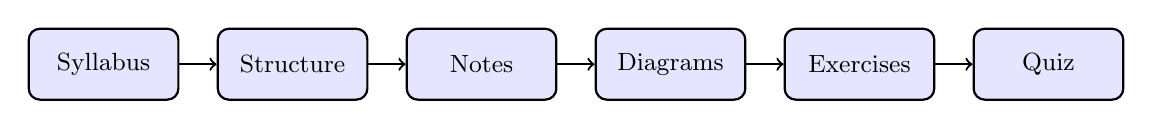
\begin{tikzpicture}[box/.style={draw, rounded corners, thick, fill=blue!10, minimum height=0.9cm, minimum width=1.9cm, align=center, font=\small}]
\node[box] (a) at (0,0) {Syllabus};
\node[box] (b) at (2.4,0) {Structure};
\node[box] (c) at (4.8,0) {Notes};
\node[box] (d) at (7.2,0) {Diagrams};
\node[box] (e) at (9.6,0) {Exercises};
\node[box] (f) at (12.0,0) {Quiz};
\foreach \x/\y in {a/b,b/c,c/d,d/e,e/f} \draw[->, thick] (\x) -- (\y);
\end{tikzpicture}}
\end{center}
\begin{itemize}
\item Each arrow is one CRAFT prompt, and each output gets your review before it moves on.
\item Work one topic fully through the pipeline first, then repeat it for the rest.
\end{itemize}
\end{frame}

%%%%%%%%%%%%%%%%%%%%%%%%%%%%%%%%%%%%%%%%%%%%%%%%%%%
\begin{frame}[fragile]\frametitle{Step 1: Syllabus to Structure}
\begin{itemize}
\item Paste your syllabus and ask for an outline that maps onto sections, subsections and units.
\end{itemize}
\begin{lstlisting}[language=HTML]
You are an experienced Grade 9 science teacher (R).
Here is my syllabus: [PASTE SYLLABUS] (C).
Propose a course outline: 5 sections, each with
3 lessons, each lesson with a one-line goal (A).
Format as a nested list, no extra commentary (T).
\end{lstlisting}
\end{frame}

%%%%%%%%%%%%%%%%%%%%%%%%%%%%%%%%%%%%%%%%%%%%%%%%%%%
\begin{frame}[fragile]\frametitle{Step 2: Expand One Topic with CRAFT}
\begin{itemize}
\item Choose one lesson from the outline and expand it fully before touching the others.
\end{itemize}
\begin{lstlisting}[language=HTML]
You are a patient Grade 9 science teacher (R).
My class knows cells and tissues (C).
Write course notes on photosynthesis: 600 words,
3 headings, 1 worked example, 2 common
mistakes (A). Match the tone of this sample:
[PASTE A PARAGRAPH YOU LIKE] (F).
Simple words, short sentences (T).
\end{lstlisting}
\end{frame}

%%%%%%%%%%%%%%%%%%%%%%%%%%%%%%%%%%%%%%%%%%%%%%%%%%%
\begin{frame}[fragile]\frametitle{Prompts for Course Notes}
\begin{itemize}
\item \textbf{Draft:} ask for notes at a stated level, length and heading structure.
\item \textbf{Adapt:} ask for the same notes at an easier level, or with local examples.
\item \textbf{Shorten:} ask for a one-page cheat sheet from the full notes.
\item \textbf{Check:} ask the AI to list claims in its own notes that you should verify.
\item Save prompts that worked in your prompt library, with placeholders for topic and grade.
\end{itemize}
\end{frame}

%%%%%%%%%%%%%%%%%%%%%%%%%%%%%%%%%%%%%%%%%%%%%%%%%%%
\begin{frame}[fragile]\frametitle{Diagrams as SVG by Prompt}
\begin{itemize}
\item SVG is text, so an AI can write it. It scales cleanly and drops straight into an HTML unit or a slide.
\item Describe the diagram, the labels and the colours; ask for SVG code only.
\item Save the reply as \texttt{water\_cycle.svg} and open it in a browser. Ask for fixes in plain words.
\end{itemize}
\begin{lstlisting}[language=HTML]
Draw an SVG, 400x200, of a water cycle:
sun top-left, cloud top-right, sea at the
bottom, arrows for evaporation and rain,
each arrow labelled. Output only the SVG code.
\end{lstlisting}
\end{frame}

%%%%%%%%%%%%%%%%%%%%%%%%%%%%%%%%%%%%%%%%%%%%%%%%%%%
\begin{frame}[fragile]\frametitle{Diagrams: Other Routes}
\begin{itemize}
\item \textbf{Mermaid or Graphviz text:} ask the AI for flowcharts and concept maps as text, then render them.
\item \textbf{draw.io or PowerPoint:} ask for a layout plan and label list, then draw by hand for full control.
\item \textbf{Image generators:} fine for illustrations, but weak at accurate labels; always check the text inside the image.
\item For science and maths diagrams, prefer text-based formats you can inspect and correct.
\end{itemize}
\end{frame}

%%%%%%%%%%%%%%%%%%%%%%%%%%%%%%%%%%%%%%%%%%%%%%%%%%%
\begin{frame}[fragile]\frametitle{Exercises with Graded Difficulty}
\begin{itemize}
\item Ask for exercises in levels, so every student finds a starting point.
\end{itemize}
\begin{lstlisting}[language=HTML]
You are a Grade 9 science teacher (R).
For the photosynthesis notes above (C), write
9 exercises: 3 routine, 3 applied, 3 challenge (A).
Give a short model answer for each (A).
Match the question style of my sample [SAMPLE] (F).
No question may need outside data (T).
\end{lstlisting}
\end{frame}

%%%%%%%%%%%%%%%%%%%%%%%%%%%%%%%%%%%%%%%%%%%%%%%%%%%
\begin{frame}[fragile]\frametitle{Quizzes with Answer Keys}
% [upgrade-deck: rewritten 2026-10-24 | Task 1b | trailing item moved above the listing]
\begin{itemize}
\item A quiz needs three outputs: the questions, the correct answers, and a short reason for each wrong option.
\item Keep the answer key in a separate file from the student view, and check each answer yourself.
\end{itemize}
\begin{lstlisting}[language=HTML]
Write 5 multiple-choice questions on
photosynthesis, 4 options each (A).
Return a table: Question | Correct | Why
the correct one is right | Why each wrong
option is wrong (T).
Mix recall and application questions (T).
\end{lstlisting}
\end{frame}

%%%%%%%%%%%%%%%%%%%%%%%%%%%%%%%%%%%%%%%%%%%%%%%%%%%
\begin{frame}[fragile]\frametitle{A Quiz Item in Open edX Format}
\begin{itemize}
\item Ask the AI to return questions as Open edX problem XML, then paste it into a Problem component in Studio.
\end{itemize}
\begin{lstlisting}[language=HTML]
<problem>
<multiplechoiceresponse>
<label>Which gas do plants take in?</label>
<choicegroup type="MultipleChoice">
<choice correct="false">Oxygen</choice>
<choice correct="true">Carbon dioxide</choice>
<choice correct="false">Nitrogen</choice>
</choicegroup>
</multiplechoiceresponse>
<solution><p>Plants take in carbon
dioxide for photosynthesis.</p></solution>
</problem>
\end{lstlisting}
\end{frame}

%%%%%%%%%%%%%%%%%%%%%%%%%%%%%%%%%%%%%%%%%%%%%%%%%%%
\begin{frame}[fragile]\frametitle{Check Before You Publish}
\begin{itemize}
\item \textbf{Facts:} verify every number, date, name and formula against your textbook.
\item \textbf{Level:} read it as a student would; shorten any sentence you stumble over.
\item \textbf{Diagrams:} check each label and arrow, and test the image on a phone.
\item \textbf{Quiz:} answer every question yourself and confirm the key matches.
\item \textbf{Privacy:} no real student names or data in any prompt sent to a public tool.
\end{itemize}
\end{frame}

\section[Activity]{Workshop Activity}

%%%%%%%%%%%%%%%%%%%%%%%%%%%%%%%%%%%%%%%%%%%%%%%%%%%
\begin{frame}[fragile]\frametitle{Activity: Your Own Course Booklet}
\begin{itemize}
\item Take one syllabus you teach, and build a first booklet in this session.
\item \textbf{Step 1:} write a CRAFT prompt that turns your syllabus into a section and lesson outline.
\item \textbf{Step 2:} pick one lesson and expand it fully with a CRAFT prompt: notes, one diagram, three exercises.
\item \textbf{Step 3:} add a five-question quiz with an answer key.
\item \textbf{Step 4:} review it against the checklist, and swap with a neighbour for comments.
\end{itemize}
\end{frame}

%%%%%%%%%%%%%%%%%%%%%%%%%%%%%%%%%%%%%%%%%%%%%%%%%%%
\begin{frame}[fragile]\frametitle{Flipped Classroom: The Takeaways}
\begin{itemize}
\item Flipping moves content delivery before class and gives class time to discussion and application.
\item Pick the lightest route that works: textbook, notes, playlist or LMS. They combine well.
\item Open edX and Moodle are both free software; the cost is in hosting and set-up, so plan for it.
\item AI drafts structure, notes, diagrams, exercises and quizzes. You decide, correct and own the result.
\end{itemize}
\end{frame}
